\subsection{Südkamerun}\label{sec:Kamerun}

Das nordwestlich an das Arbeitsgebiet angrenzende südliche Kamerun zählt, neben dem Norden Gabuns (Kap.~\ref{sec:Gabun}) sowie dem Niederkongo (Kap.~\ref{sec:Niederkongo}), gegenwärtig zu den archäologisch bester erforschten Regionen in Zentralafrika.\footnote{Zur Geschichte der archäologischen Erforschung Südkameruns siehe auch \textcite[7--9]{Seidensticker.2010b}.} Archäologische Forschungen in Kamerun konzentrierten sich lange Zeit auf das Zentrum des Landes und rückten vornehmlich die keramischen Formen des Fundplatzes Obobogo in den Mittelpunkt der Betrachtungen. Während die Fundstelle in den 1940er Jahren durch \mbox{J.-B.} \textcites{Jauze.1944}{Jauze.1944b}{Jauze.1948} entdeckt wurden, fanden ab den 1980er Jahren systematische Grabungen unter der Leitung von \mbox{Pierre} \textcites{Maret.1980}{Maret.1982} in Obobogo statt.\footnote{Neben den Feldarbeiten im Umland von Yaoundé wurden unter der Leitung von \textcites{deMaret.1995}{Maret.1996} eine Reihe von Abris im Westen Kameruns, genauer gesagt in den sogenannten \textit{Grassfields}, untersucht. Dabei konnte an der Fundstelle Shum Laka eine der umfangreichsten, vom späten Pleistozän bis ins Holozän reichende Sequenz erfasst werden \parencites{Asombang.1988}{Asombang.1992}{deMaret.1995}{Maret.1996}{Lavachery.1996}{Moeyersons.1996}{Cornelissen.1996}{Cornelissen.2003}. Die ursprünglich mikrolithische \textit{Later Stone Age} (LSA), Steingeräteindustrie dieses Platzes wandelt sich im 5. Jt. v.~Chr. sukzessive zu einer makrolithischen Industrie. Daneben finden sich erstmals geschliffene Steinwerkzeuge und eindruck-verzierte Keramik \parencite[225, 243]{Lavachery.2001}. Der Beginn dieser Entwicklung wird von \textsc{Lavachery} (ebd. 243) unter dem Terminus \textit{Ceramic Late Stone Age} systematisiert, die in eine, in Anlehnung an \textcite{McIntosh.1988}, als \textit{Stone to Metal Age} \parencite[SMA;][213]{Lavachery.2001} beziehungsweise \textit{Stone to Metal Period} \parencite[SMP;][279]{Maret.1996} bezeichnete, mutmaßlich eigenständige Kulturerscheinung münden soll. Die Bezeichnung \textit{Neolithikum} wird explizit vermieden, da direkte Belege für produzierende Wirtschaftsweise fehlen \parencite[243]{Lavachery.2001}. Die Formen dieser Phase haben im Inventar von Shum Laka bis zum Beginn der Eisenzeit im 4.~Jh. v.~Chr. bestand \parencite[278]{Maret.1996}. Die Keramik der obersten, klar eisenzeitlichen, aber stark durchmischten Schicht zeichnet sich durch \textit{knotted strip}- (Tab.~\ref{tab:Verzierungselemente}: 21.1) sowie \textit{twisted string}-Roulette (Tab.~\ref{tab:Verzierungselemente}: 21.2) aus.\label{ftn:ShumLaka}} Durch \textcite{Claes.1985} erfolgte lediglich eine grobe Aufarbeitung der Keramik, so dass gesicherte Aussagen nur bedingt möglich sind. In den späten 1980er und frühen 1990er Jahren  wurden im Umland von Yaoundé weiterer Fundstellen entdeckt und untersucht \parencite{Essomba.1989}. Im Zuge der neuen Feldarbeiten entstanden eine Reihe von Promotionsschriften: Christine \textcite{Atangana.1988} zur Fundstelle Okolo, die Arbeit von Christoph \textcite{MbidaMindzie.19951996} über die Fundstellen Nkang und \mbox{Ndindan} sowie die Bearbeitung mehrerer Fundstellen südlich des Sanaga durch Martin \textcite{Elouga.20002001}. Die in Okolo, Nkang und Ndindan gefundene Keramik weist starke Parallelen zu den in Obobogo gefundenen Formen. Diese bilden den Beginn der regionalen keramischen Sequenz ab. Es handelt sich dabei um hohe, flachbodige Gefäße mit leicht geschweiften Wandungen sowie Wiegebandverzierung und gerillten Rändern \parencite[Abb.~\ref{fig:swCameroon_Sequence}.1--4;][]{Claes.1985}. Die Verzierungen sind häufig flächig über alle Gefäßteile hinweg zu finden. Neben der Keramik fanden sich auch Steinartefakte sowie Schlacke, was zumindest \enquote{eine Phase gleichzeitiger Verwendung lithischer und metallener Gerätschaften} andeutet \parencite[258\,f.]{Wotzka.1995}. Die vorliegenden absoluten Datierungen aus Obobogo weisen starke Abweichungen auf und ohne eine zufriedenstellende Vorlage der Befunde lassen sich aus ihnen nur sehr begrenzt chronologische Rückschlüsse ziehen.\footnote{Viele der vorliegenden Radiokohenstoffdatierungen aus Obobogo wurden im Labor in Hannover untersucht und weisen ähnlich starke Schwankungen auf, wie die Datierungen aus dem Inneren Kongobecken (siehe Kap.~\ref{sec:ICB_StilGrDatierungen}). Auch wurde für die konventionellen Radiokohlenstoffdatierungen in den 1980er Jahren regelhaft Probenmaterial zu sogenannten \textit{bulk samples} vermischt, um ausreichend datierbares Material zu erhalten \parencite[723]{Clist.20042005}. Die vorliegenden Daten streuen zwischen dem 24.--16.~Jh. v.~Chr. (Hv-11046) sowie dem 2.~Jh. v.~Chr.--2.~Jh. n.~Chr. \parencites[Hv-10832;][147]{deMaret.1985b}[219\,f.]{Clist.1986}[nach][249 Anm. 21]{Wotzka.1995}. Von den insgesamt 13 Datierungen wurden nur drei nicht in Hannover untersucht (Lv-1394, Lv-1395, Lv-1432). Diese drei Datierungen decken eine Zeitspanne vom 8.~Jh. v.~Chr. bis zum 3.~Jh. n.~Chr. ab.}

\begin{figure*}[p]
	\centering
	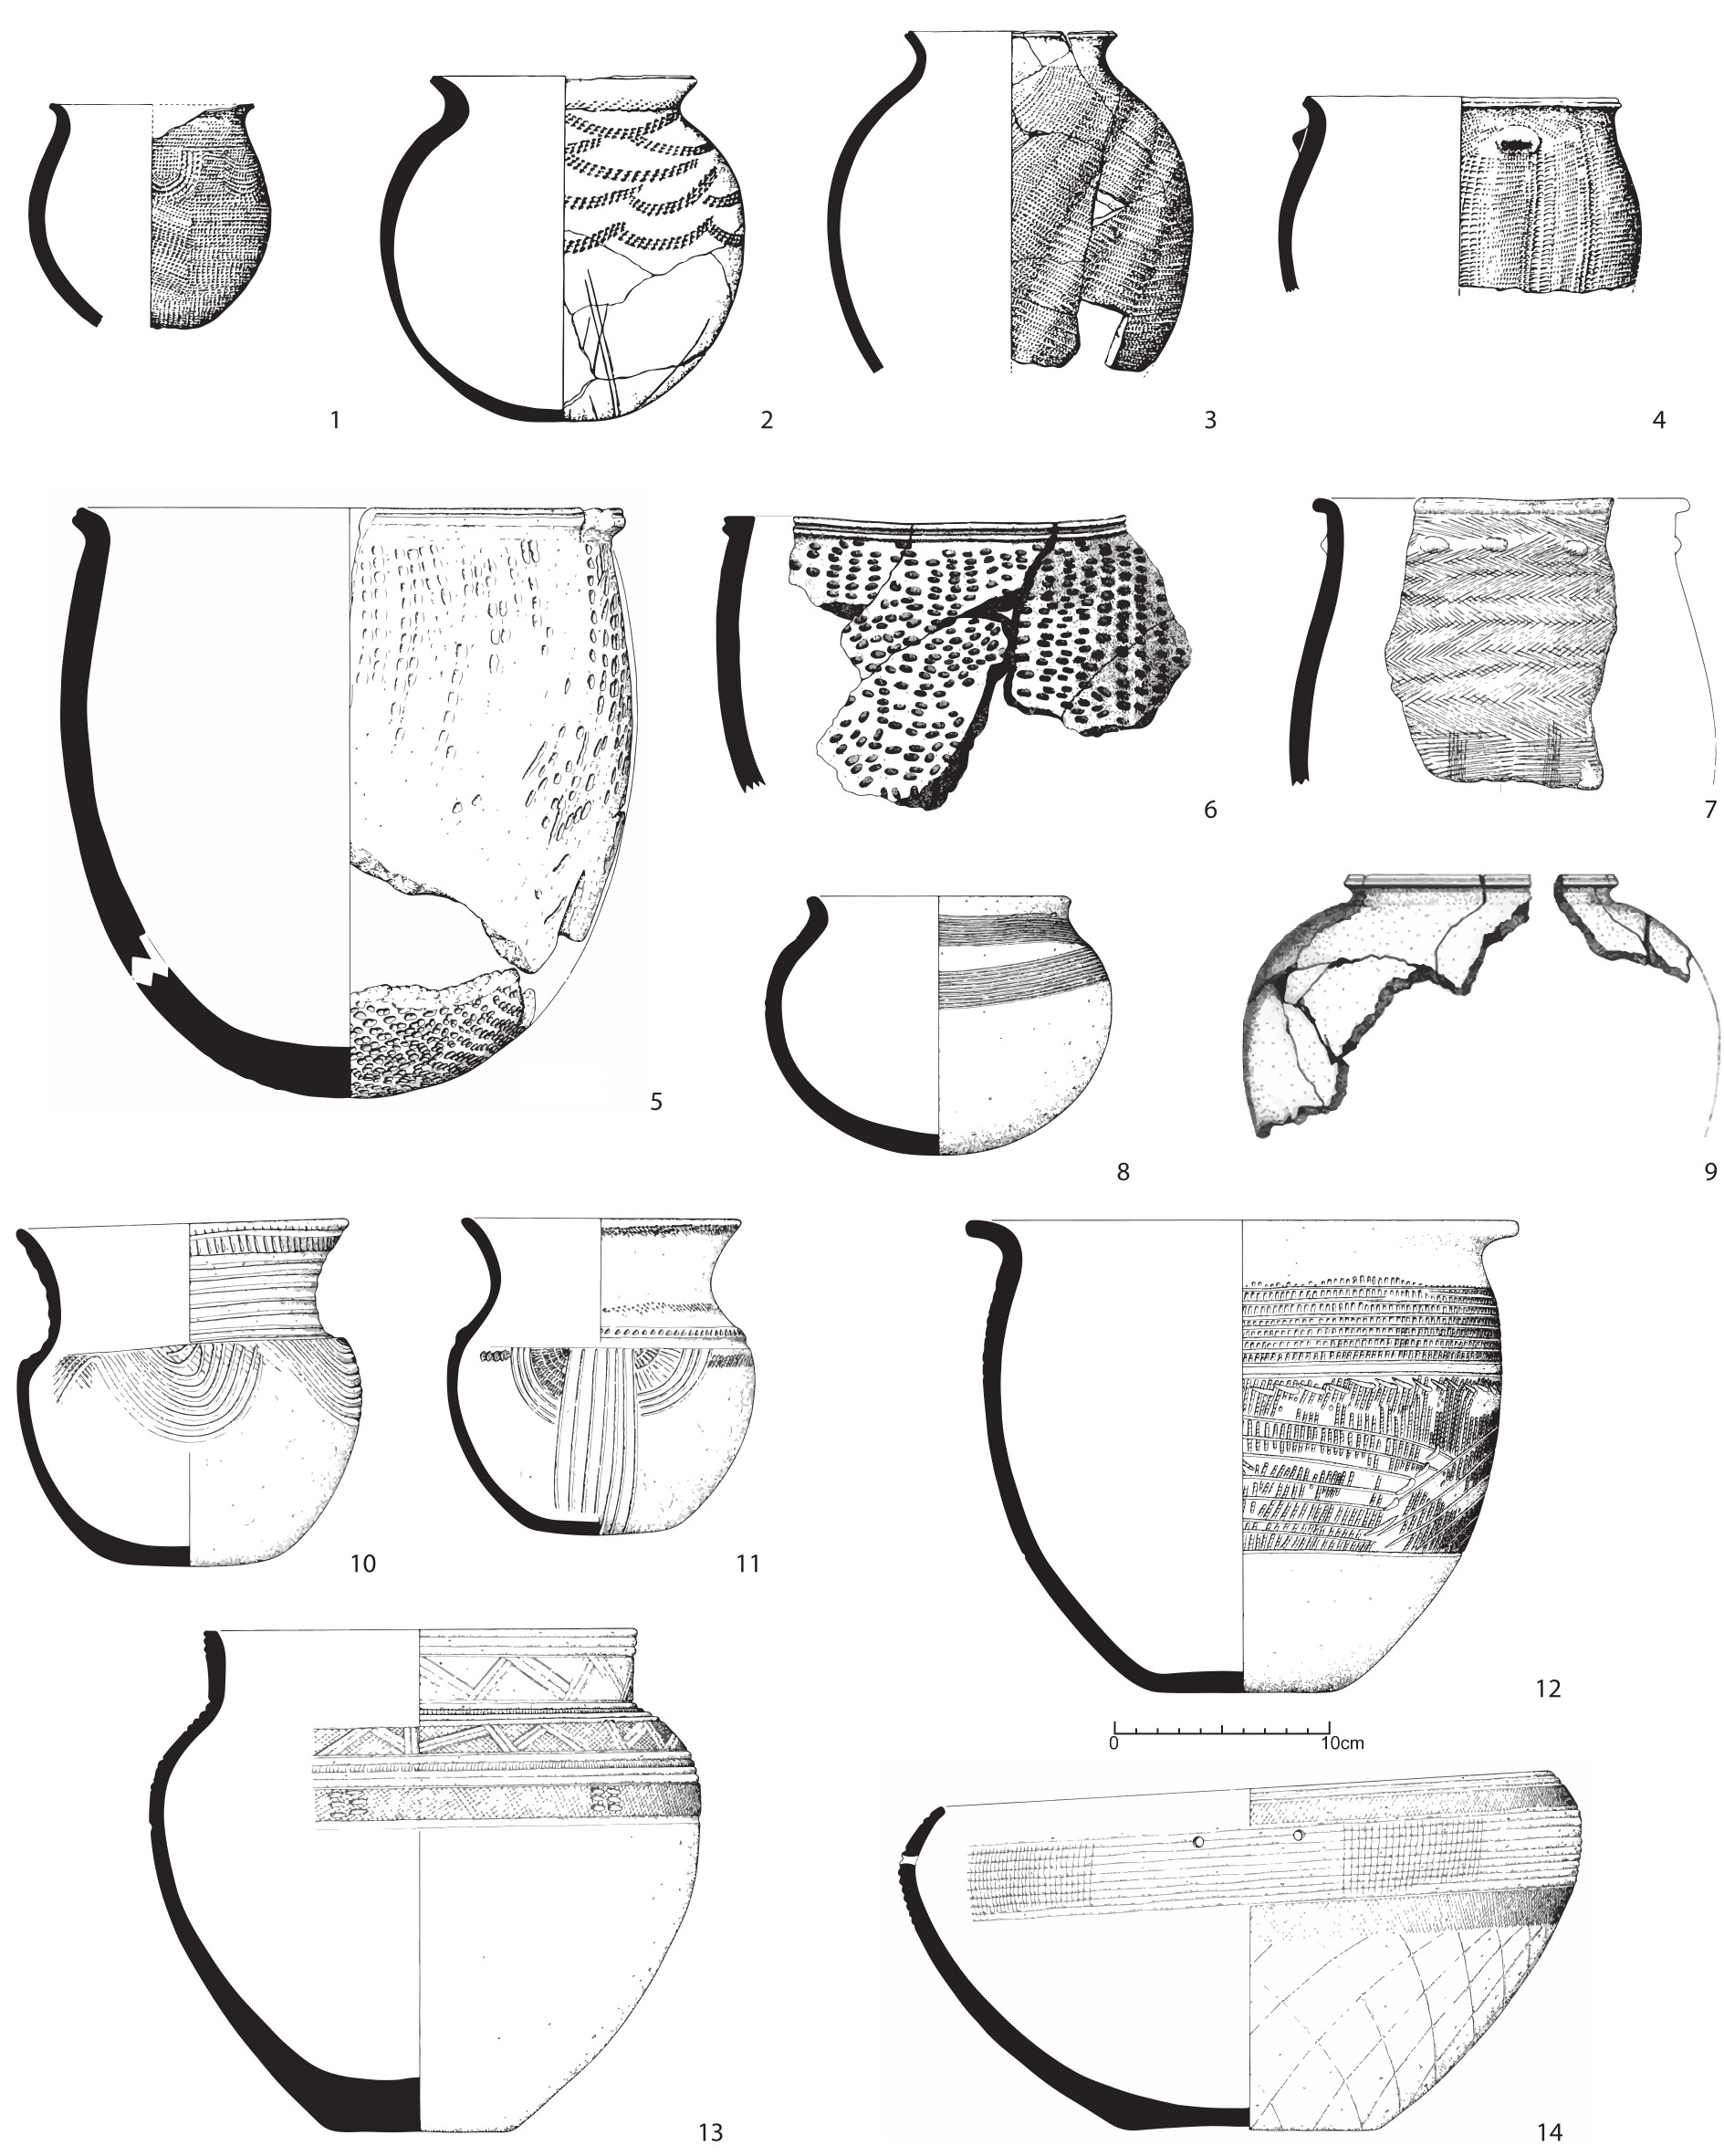
\includegraphics[width = \textwidth]{fig/Kamerun_Typen.pdf}
	\caption{Südliches Kamerun: Regionale Sequenz der frühen Eisenzeit nach \textcites{GouemGouem.20102011}{NlendNlend.20132014}.\\ 1--4: Obobogo-Gruppe \parencites[Taf. 25.1--2, 37.1, 39.2]{Claes.1985}[632 Abb.~43.4]{deMaret.2013}; 5--7: Bissiang/Malongo-Gruppe \parencites[34 Abb.~14]{Oslisly.2001c}[282 Abb.~3.2, 287 Abb.~7.3]{Eggert.2006b}; 8--9: Mpoengu/Bwambé-Gruppe \parencites[282 Abb.~3.7]{Eggert.2006b}[252 Abb.~114.2]{NlendNlend.20132014}, 10--13: Akonètye (Nord) \parencite[195 Abb.~10.2--5]{Meister.2008b}; Akonètye (Süd) (ebd. 188 Abb.~5.2); 13--14: Campo-Gruppe \parencite[98 Abb.~5.6, 182 Taf.~12.2, 184 Taf.~14.4]{Eggert.2016}.}
	\label{fig:swCameroon_Sequence}
\end{figure*}

Der an das Arbeitsgebiet anschließende Südosten Kameruns\footnote{Die archäologischen Funde neuerer Forschungsaktivitäten in der Region \parencite{MorinRivat.2014} sind gegenwärtig nicht abschließend vorgelegt.} hat im Vergleich zum Zentrum des Landes sowie dem Südwesten vergleichsweise wenig Forschungsaktivität erfahren. 1997 nahm \textcite{Eggert.2002} die in dieser Arbeit präsentierten Feldarbeiten im Norden der Republik Kongo, entlang der Flüsse \mbox{Sangha} und \mbox{Ngoko}, durch Prospektionen im Südosten Kameruns wieder auf.\footnote{Aufgrund aufschlussreicher Funde entlang des Sanaga verschoben sich die Prioritäten folgender Feldarbeiten sukzessive in den Südwesten Kameruns. So wurden 1998/99 umfangreiche Grabungen im nahe der Mündung des Sanaga gelegenen Mouanko durchgeführt (\textsc{Eggert} 2002). Das ebenfalls unter der Leitung von Manfred Eggert durchgeführte Teilprojekt in Kamerun, der 2004 begründeten DFG-Forschergruppe 510 \enquote{Ökologischer Wandel und kulturelle Umbrüche in West- und Zentralafrika} der Universitäten Frankfurt am Main und Tübingen, führte schließlich zu umfangreichen Feldarbeiten in Südkamerun. Die Auswertung der Befunde und Funde, die im Zuge dieses Projektes erschlossen wurden, steht gegenwärtig noch aus.} Gegenwärtig informiert lediglich ein knapper Vorbericht über die Ergebnisse der Prospektionen des Tübinger Projektes im Südosten Kameruns (ebd. 510\,f.). Die Region um Moloundou am \mbox{Ngoko} erwies sich als äußerst spärlich besiedelt. Eine deutlich dichtere Besiedlung zumindest in historischer Zeit deuten für die Region verfügbare Karten an, die auf Basis von Luftaufnahmen erstellt wurden und häufig Vermerke von Ölpalmen aufweisen (ebd.).\footnote{Diese können als indirekte Anzeiger für potenzielle menschliche Aktivitäten angesehen werden. Ölpalmen (\textit{Elaeis guineensis}) finden sich in vielen archäologischen Fundstellen Kameruns und bilden einen allgemeinen Anzeiger für lichtreichere Sekundärwälder \parencite{Neumann.2006}. Zur Bedeutung der Ölpalme in Westafrika siehe auch \textcites{Sowunmi.1999}{DAndrea.2006}{Logan.2012}.} Aufgrund hoher Wasserstände erbrachte die Prospektion des Jahres 1997 im Südosten Kameruns keine Hinweise auf frühe Keramik.\footnote{Eine begrenzte Anzahl von kleinen Schälchen mit T-förmigen Rändern, die im Zuge dieses Surveys gefunden wurden und deutliche Parallelen zu den Inventaren der Stilgruppen Konda und Pandama (Kap.~\ref{sec:KON-Gr}--\ref{sec:PDM-Gr}) zeigen, weisen auf Beziehungen zwischen dem oberen \mbox{Sangha}-/\mbox{Ngoko}-Gebiet und Südostkamerun sowie eine potenzielle Anbindung dieses Raumes an die \textit{\mbox{Ngoko}-Tradition} (Kap.~\ref{sec:NgokoTradition}) hin. Siehe auch Anm.~\ref{ftn:KON-PDM_klSchalen} und \ref{ftn:SOKamerun1997Funde}.}

Die in den letzten Jahrzehnten wohl am besten untersuchte Region Kameruns ist der Südwesten des Landes, genauer das Umland von Kribi sowie der Küstenabschnitt zwischen Kribi und Campo. Vor allem die im Zuge der Errichtung der die Erdölfelder in Kome (Tschad) mit Kribi verbindenden Erdölpipeline\footnote{Die Arbeiten des Pipeline-Projektes erbrachten zahlreiche neue Fundstellen entlang eines knapp 1100\,km langes Transektes. Im Zuge dieser Zusammenstellung flossen lediglich die Funde aus dem südwestlichen Kamerun ein \parencites[siehe][]{Lavachery.2005}{Lavachery.2010}.} durchgeführten Surveys sowie Prospektionen und Grabungen unter der Leitung von Richard Oslisly\footnote{Siehe \textcites{Oslisly.2006}{Oslisly.2006d}.} und solche des Tübinger Kamerun-Projektes \parencites{Eggert.2006b}{Meister.2008b} verdichteten die archäologische Karte des südwestlichen Kameruns merklich. Im Zuge der Promotionsarbeiten von Bienvenu \textcite{GouemGouem.20102011} und Pascal \textcite{NlendNlend.20132014} kam es zu einer abweichenden nomenklatorischen Beschreibung der jeweils gleichen archäologischen Phänomene. Die ältesten keramischen Zeugnisse werden von \textcite[330--341]{GouemGouem.20102011} der Bissiang-Gruppe zugerechnet, während die gleichen Formen von \textcite[233--249]{NlendNlend.20132014} einer Malongo genannten Gruppe zugewiesen werden. Die entsprechende Keramik zeichnet sich durch hohe, ovaloide Gefäße mit flächiger Fischgrät-Verzierung, Kammwiegeband sowie häufig kurz ausbiegenden, gerillten Rändern aus \parencites[337 Abb.~11.6]{GouemGouem.20102011}[237--239 Abb.~102--104; Abb.~\ref{fig:swCameroon_Sequence}.5--7]{NlendNlend.20132014}. Vertreter dieser Keramik fanden sich in Bissiang, Dombè, Malongo, Bwambé-Sommet, Abang Minko'o, Mpolongwé-Kribi und Campo \parencites[336, 339 Karte 1.6]{GouemGouem.20102011}[254]{NlendNlend.20132014}{Seidensticker.2010b}. \textcite[336 Abb. 10.6]{GouemGouem.20102011} gibt für die Bissiang-Gruppe auf Basis von je zwei Datierungen aus Bissiang (Beta-182548, Beta-182549) und Dombè (Beta-182546, Beta-182547) ein Alter zwischen dem 11.--4. Jh. v.~Chr. an, wobei ohne die älteste Probe (Beta-182549) lediglich eine Spanne zwischen dem \mbox{8.--4. Jh.} v.~Chr. unterstützt ist (ebd. 336 Abb. 10.6). Für die der Bissiang-Keramik entsprechende Malongo-Gruppe werden von \textcite[255 Abb.~116]{NlendNlend.20132014} zwölf Datierungen genannt, die einen Zeitraum vom 11.~Jh. v.~Chr. bis in das 1.~Jh. v.~Chr. abdecken. Die Malongo-Gruppe wird von \textsc{Nlend Nlend} (ebd. 247) als Teil der vielgestaltig systematisierten, ähnlich frühen Keramik in Kamerun und Gabun angesehen. \textcite[632 Abb.~43.3]{deMaret.2013} fasst diese unterschiedlich bezeichneten Gruppen, die jedoch alle mehr oder weniger das gleiche keramische Phänomen abbilden, gemeinsam unter der Bezeichnung \enquote{Diverse verwandte Traditionen} zusammen.

Des Weiteren beschreibt \textcite[254--257]{NlendNlend.20132014} einen ab dem frühen 7.~Jh. v.~Chr. aufkommenden Stil, den er als Bwambé-Gruppe bezeichnet. Das Formenspektrum entspricht dabei den von \textcite[352--358, 354 Abb.~17.6]{GouemGouem.20102011} als Mpoengu-Gruppe subsumierten Inventaren. Beide zeichnen sich durch rundbauchige Gefäße mit in horizontalen Bändern organisierten Verzierungen und kurzen, ausbiegenden Rändern aus \parencite[ebd. 352--358, 354 Abb.~17.6; ][252 Abb.~114; Abb.~\ref{fig:swCameroon_Sequence}.8--9]{NlendNlend.20132014}. Während \textcite{GouemGouem.20102011} diese Funde an den Beginn der regionalen Eisenzeit stellt\footnote{\textsc{Gouem Gouem} (2010/2011: 349\,f.) setzt den Beginn der Eisenzeit im südwestlichen Kamerun um 400 v.~Chr. an und führt als Beleg Funde eines Ofens aus Makouré~I sowie Fragmente von Tuyères aus Kpwé-Monekpwé an. Ebenfalls in die Frühe Eisenzeit, die mit einem Bruch in der Sequenz einhergehen, werden von \textsc{Gouem Gouem} (ebd. 350) Funde aus Talla (TAL~II-BK), Mpoengu (MPO-I-A) sowie Bwambé (Bwambé-Est) eingeordnet.}, die bei ihm erst im 4. Jh. v.~Chr. beginnt (ebd. 349\,f.), repräsentiert die Bwambé-Gruppe bei \textcite{NlendNlend.20132014} noch einen Zustand, der er einer \textit{Stone to Metal Age} (SMA) zuordnet. Die Bwambé-Keramik wird von \textsc{Nlend Nlend} (ebd. 256 Abb.~117) bis in das frühe 2. Jh. n.~Chr. datiert, während die von ihm beschriebene, ältere Malongo-Gruppe bis in das späte 1. Jh. v.~Chr. bestanden haben soll (ebd. 255 Abb.~116). Auffällig in der Analyse von \textcite{NlendNlend.20132014} ist der hohe Anteil durchmischter Inventare.\footnote{Sieben Gruben weisen ausschließlich Keramik auf, die von \textsc{Nlend Nlend} (2013/2014: 257 Tab.~44) der Malongo-Gruppe zugerechnet wird (Bissiang A und B; Dombé A und B, Malongo 2 sowie Mpolongwé-Kribi 15 und 22), während sieben Gruben ausschließlich Material der Bwambé-Gruppe enthalten (Bwambé 1, 2, 4, 9 und 11 sowie Mpoengu I-A und Talla II BK). Elf weitere Gruben enthalten Formen beider Gruppen (Bwambé 12, 16, 17, 19, 32, 33 und 34 sowie Mpolongwé-Kribi 8, 23, 31 und 36). \textsc{Nlend Nlend} (ebd.) wertet die Inventare aus den Gruben 1 und 2 in Bwambé, die beide jeweils 97,99\,\% beziehungsweise 86,19\,\% Keramik der Bwambé-Gruppe enthalten, als durchmischt, während Inventare mit deutlich geringeren Anteilen Malongo-Keramik vollständig dieser zugerechnet werden. Hierzu zählen die Inventare aus den Gruben 16 (47,05\,\% Malongo-Keramik), 17 (68,6\,\% Malongo-Keramik) und 19 aus Bwambé, die nur 27,53\,\% Malongo-Keramik enthielt. Die daraus notwendigen Anpassungen sind in die weiter oben genannten Zahlen eingeflossen. Bereits im Inventar aus Grube 31 in Mpolongwe-Kribi, welches in das 9.--7.~Jh. v.~Chr. datiert und zu den ältesten datierten Grubeninventaren der von \textcite{GouemGouem.20102011} und \textcite{NlendNlend.20132014} untersuchten Region gehört, findet sich Keramik, die von \textsc{Nlend Nlend} (ebd. 257 Tab.~44) der Bwambé-Gruppe zugerechnet wurde. Auch die ins 9.--5.~Jh. v.~Chr. datierte Grube 17 aus Bwambé enthält knapp ein Drittel nicht der Malongo-Gruppe zurechenbare Funde.}

Eine zweite, entwickeltere Phase der frühen Eisenzeit sieht \textcite[363--369, 368 Abb.~30.6]{GouemGouem.20102011} durch die Keramik der Bidjouka-Gruppe repräsentiert, die tief in die Oberfläche eingearbeitete, im Profil U-förmige Riefen sowie Kammwiegeband aufweist. Dieser Stil datiert zwischen das 1.--7.~Jh. n.~Chr. (ebd. 371 Abb.~33.6) und ist zeitgleich mit der Belegung des Gräberfeldes in Campo und der dort angetroffenen Keramik, die eine eigene Stilgruppe repräsentiert \parencite[98 Abb.~5.6]{Eggert.2016}. Die in das 1. Jh. v.~Chr. bis 3. Jh. n.~Chr. datierenden, 1998/99 an der Mündung des Sanaga ausgegrabenen Befunde aus Mouanko-Lobethal, dem benachbarten Mouanko-Epolo sowie dem auf der gegenüberliegenden Flussseite gelegenen Yatou\footnote{In Mouanko-Lobethal wurde unter anderem ein aus neun sich überlagernden Gruben bestehender Komplex sowie vier weitere Gruben untersucht \parencite[513]{Eggert.2002}.} erbrachten keramische Inventare, die Ähnlichkeiten zur Keramik der Gräber in Campo \parencites[239 Abb.~2]{Meister.2010}[98 Abb.~5.6]{Eggert.2016} sowie einer zeitgleichen Grube aufweisen \parencite[161 Abb.~3.5--10]{Seidensticker.2010c}. Diese Inventare zeichnen sich durch offene Schalenformen sowie Gefäße mit geschweifter Wandung, kurzem Hals und ausbiegenden Rändern aus \parencite[514--519 Abb.~7--12; Abb.~\ref{fig:swCameroon_Sequence}.13--14]{Eggert.2002}. Die Verzierung setzt sich vornehmlich aus Rillen oder Riefen sowie Kammeindrücken zusammen. Gefäße aus Grube 1 der am südlichen Ufer des Sanaga gelegenen Fundstelle Yatou (ebd. 519 Abb.~12.2--3) weisen hingegen schwache Ähnlichkeiten zur den diagnostischen Schalen der Pikunda-Munda-Gruppe auf (Kap.~\ref{sec:PKM-Gr}).\footnote{Wie diese haben die Gefäße aus Yatou einen scharfen Knick zwischen Ober- und Unterteil und einen runden Boden. Die Verzierung besteht wie bei der Pikunda-Munda-Gruppe aus horizontalen Bändern, wobei die Gefäße aus Yatou vornehmlich Kammeindrücke, in einem Fall ein aus einzelnen horizontalen Kammeindruck-Bändern gebildetes Fischgrätmuster, aufweisen und die Gefäßunterteile unverziert bleiben. Die Randgestaltung lässt wieder verstärkt Parallelen zwischen der Keramik aus Yatou und jener der Pikunda-Munda-Gruppe erkennen: die grundsätzlich ausbiegenden Ränder weisen eine auch bei der Pikunda-Munda-Keramik beobachtbaren, einbiegenden Randlippen auf (siehe Taf.~41.18, 45.2, 50.7, 52.6 und \textsc{Eggert} (2002: 519 Abb.~12.2--3).}

Der jüngere Abschnitt der Älteren Eisenzeit im südwestlichen Kamerun, im Anschluss an die Mpoengu-Gruppe, wird von \textcite[379\,f.]{GouemGouem.20102011} in zwei Phasen unterteilt: eine erste vom 1.--4.~Jh. n.~Chr. datierende Phase mit Funden in Akonétyé, Minyin, Mouanko-Lobethal sowie Campo und eine zweite Phase, die zwischen das 4.--10.~Jh. n.~Chr. datiert und zu der Funde aus Bidjouka, Kribi-Mission catholique, Talla, Mpoengu, Eboundja 3, Bidou I, Bwambé Beach und Boussibilinga gezählt werden.\footnote{Eine in Mpoengu freigelegte Bestattung datiert in diese zweite Phase (\textsc{Gouem Gouem} 2010/2011: 305--317, 384--389).} Zur ersten Phase zählt \textsc{Gouem Gouem} (ebd.) auch die in das 1.--4.~Jh. n.~Chr. datierenden Funde aus dem am Mboro-Fluss nördlich von Ambam gelegenen Akonétye \parencite[184]{Meister.2008b}. Die untersuchten Bereiche der Fundstellen erbrachten nahezu zeitgleiche Gruben, jedoch zeigen sich zwischen den keramischen Inventaren der nördlichen sowie der südlichen Fundstellen deutliche formale Unterschiede. Die Gruben der südlichen Fundstelle waren zwischen 0,5--3,9\,m tief und enthielten Keramik, die sich durch hohe, leicht geschweifte Grundformen mit flachen Böden und ausbiegenden Rändern auszeichnet (Abb.~\ref{fig:swCameroon_Sequence}.12; ebd. 188 Abb.~5). Die Stücke sind vor allem mittels horizontal um die Gefäße laufenden, breiten in Wiegebandtechnik erzeugten Bändern sowie Rillen und kleineren Eindruck-Reihen verziert. Die fast zeitgleiche nördliche Fundstelle erbrachte eine komplett andersartige Keramik: gedrungenere Gefäße mit geschweifter Wandung und auffälligem Schulterabsatz. Ihre Verzierungen bestehen aus horizontalen Rillen an vornehmlich langen, konvexen Halsbereichen sowie bogen- beziehungsweise girlandenförmigen Rillenbündeln unterhalb der Schulterabsätze (Abb.~\ref{fig:swCameroon_Sequence}.10--11; ebd. 195 Abb.~10). Die jeweiligen Grubeninventare der beiden Fundstellen von Akonétye sind formal in sich äußerst homogen, unterscheiden sich untereinander aber diametral. Der Keramik der nördlichen Fundstelle aus Akonétye entsprechendes Material fand sich auch im zirka 20\,km entfernt gelegenen Minyin (\textsc{Meister \& Eggert} 2008: 196 Abb.~11)\footnote{Die Funde aus Minyin datieren in das 1. Jh. v.~Chr. bis 3. Jh. n.~Chr. (\textsc{Meister \& Eggert} 2008: 189 Tab.~1).} sowie östlich von Sangmélima in Akom \parencite[413 Abb.~6.1,10]{deSaulieu.2015}. In der gleichen Region wurde an einer Reihe von Orten zudem Keramik gefunden, die jener der südlichen Fundstelle von Akonétye entspricht (ebd.~410 Abb.~5). Die jüngeren Abschnitte der Keramiksequenz im südlichen Kamerun sind bislang kaum Gegenstand von archäologischer Forschung gewesen. Lediglich der von \textcite{Elouga.20002001} verfolgte ethno-archäologische Ansatz bei der Auseinandersetzung mit der Keramik der Region zwischen Yaoundé und dem Sanaga schloss auch die rezente Töpfereitradition mit ein. Jüngere keramische Formen sind überdies nur kursorisch beschriebe, so aus Dibamba, südlich von Douala \parencite{Saulieu.2017}.